\documentclass[]{article}
\usepackage[T1]{fontenc}
\usepackage{lmodern}
\usepackage{amssymb,amsmath}
\usepackage{ifxetex,ifluatex}
\usepackage{fixltx2e} % provides \textsubscript
% use upquote if available, for straight quotes in verbatim environments
\IfFileExists{upquote.sty}{\usepackage{upquote}}{}
\ifnum 0\ifxetex 1\fi\ifluatex 1\fi=0 % if pdftex
  \usepackage[utf8]{inputenc}
\else % if luatex or xelatex
  \ifxetex
    \usepackage{mathspec}
    \usepackage{xltxtra,xunicode}
  \else
    \usepackage{fontspec}
  \fi
  \defaultfontfeatures{Mapping=tex-text,Scale=MatchLowercase}
  \newcommand{\euro}{€}
\fi
% use microtype if available
\IfFileExists{microtype.sty}{\usepackage{microtype}}{}
\usepackage[margin=1in]{geometry}
\usepackage{color}
\usepackage{fancyvrb}
\newcommand{\VerbBar}{|}
\newcommand{\VERB}{\Verb[commandchars=\\\{\}]}
\DefineVerbatimEnvironment{Highlighting}{Verbatim}{commandchars=\\\{\}}
% Add ',fontsize=\small' for more characters per line
\usepackage{framed}
\definecolor{shadecolor}{RGB}{248,248,248}
\newenvironment{Shaded}{\begin{snugshade}}{\end{snugshade}}
\newcommand{\KeywordTok}[1]{\textcolor[rgb]{0.13,0.29,0.53}{\textbf{{#1}}}}
\newcommand{\DataTypeTok}[1]{\textcolor[rgb]{0.13,0.29,0.53}{{#1}}}
\newcommand{\DecValTok}[1]{\textcolor[rgb]{0.00,0.00,0.81}{{#1}}}
\newcommand{\BaseNTok}[1]{\textcolor[rgb]{0.00,0.00,0.81}{{#1}}}
\newcommand{\FloatTok}[1]{\textcolor[rgb]{0.00,0.00,0.81}{{#1}}}
\newcommand{\CharTok}[1]{\textcolor[rgb]{0.31,0.60,0.02}{{#1}}}
\newcommand{\StringTok}[1]{\textcolor[rgb]{0.31,0.60,0.02}{{#1}}}
\newcommand{\CommentTok}[1]{\textcolor[rgb]{0.56,0.35,0.01}{\textit{{#1}}}}
\newcommand{\OtherTok}[1]{\textcolor[rgb]{0.56,0.35,0.01}{{#1}}}
\newcommand{\AlertTok}[1]{\textcolor[rgb]{0.94,0.16,0.16}{{#1}}}
\newcommand{\FunctionTok}[1]{\textcolor[rgb]{0.00,0.00,0.00}{{#1}}}
\newcommand{\RegionMarkerTok}[1]{{#1}}
\newcommand{\ErrorTok}[1]{\textbf{{#1}}}
\newcommand{\NormalTok}[1]{{#1}}
\usepackage{graphicx}
% Redefine \includegraphics so that, unless explicit options are
% given, the image width will not exceed the width of the page.
% Images get their normal width if they fit onto the page, but
% are scaled down if they would overflow the margins.
\makeatletter
\def\ScaleIfNeeded{%
  \ifdim\Gin@nat@width>\linewidth
    \linewidth
  \else
    \Gin@nat@width
  \fi
}
\makeatother
\let\Oldincludegraphics\includegraphics
{%
 \catcode`\@=11\relax%
 \gdef\includegraphics{\@ifnextchar[{\Oldincludegraphics}{\Oldincludegraphics[width=\ScaleIfNeeded]}}%
}%
\ifxetex
  \usepackage[setpagesize=false, % page size defined by xetex
              unicode=false, % unicode breaks when used with xetex
              xetex]{hyperref}
\else
  \usepackage[unicode=true]{hyperref}
\fi
\hypersetup{breaklinks=true,
            bookmarks=true,
            pdfauthor={梁祐誠},
            pdftitle={離散形データ研究におけるメタ解析},
            colorlinks=true,
            citecolor=blue,
            urlcolor=blue,
            linkcolor=magenta,
            pdfborder={0 0 0}}
\urlstyle{same}  % don't use monospace font for urls
\setlength{\parindent}{0pt}
\setlength{\parskip}{6pt plus 2pt minus 1pt}
\setlength{\emergencystretch}{3em}  % prevent overfull lines
\setcounter{secnumdepth}{0}

\title{離散形データ研究におけるメタ解析}
\author{梁祐誠}
\date{2014年6月27}

\begin{document}

\begin{center}
\huge 離散形データ研究におけるメタ解析 \\[0.2cm]
\large \emph{梁祐誠}\\[0.1cm]
\large \emph{2014年6月27} \\
\normalsize
\end{center}


{
\hypersetup{linkcolor=black}
\setcounter{tocdepth}{2}
\tableofcontents
}
各研究から得られた結果が出来事の比率(event
rate)のような離散形データの場合も多くのメタ解析法が提案されている。最もよく知られた方法は
Peto法(Yusuf et. al., 1985)と DerSimonian-Laird法(DerSimonian and Laird,
1986)がある。Peto法は各分割表のデータを合わせる
Mental-Haenzel法を拡張し、各研究から得られたオッツ比(odds
ratio)の推定値とその推定値の標準偏差を結合する方法である。DSL(DerSimonian-Laird)法は各研究の処理群と対照群の出来事の比率の差に基づく。2つの方法の最も大きい違いは、各研究の割り当てる重みを求めるときに、Peto方は研究内の変動(within-study
variation)だけを考慮するが、DSL方は研究間の変動(among-study
variation)も考慮することである。

\subsection{Peto法}\label{peto}

Peto法は複数の分割表からデータを結合するための
Mentel-Haenzel法を修正したものである。$i$番目の研究($i = 1, \cdots, K$)から$N$名の患者さんがあり、各研究では処理群と対照群があるとする。また、処理群には$n_i$名があり、すなわち、対処群には$N_i - n_i$名がいるとする。2つのグルプの全体で$d_i$の出来事(event)があり、処理群では$O_i$の出来事(対処群では$d_i - O_i$の出来事がある)があるとする。処理の効果がないと仮定するとき、処理群でおこる出来事の期待値は
$E_i = (n_i/N_i)d_i$である。$N_i, n_i, d_i$が与えられると$O_i$が超幾何分布(
hypergeometric
distribution)に従うことを用いて、処理効果がないという帰無仮説のもとで$O_i - E_i$は平均が0、分散が$V_i = E_i[(N_i - n_i)/N_i][(N_i - d_i)(N_i -1)]$になることを導くことができる。従って、検定統計量である

\[
\frac{\left[ \sum_{i=1}^K (O_i - E_i) \right]^2}{\sum_{i=1}^K V_i}
\]

は近似的に自由度1の$\chi^2$分布に従う。$K$個の研究から結合(pooled)されたオッツ比の推定値は
\[
\widehat{OR} = exp \left[ \frac{\sum_{i=1}^K (O_i - E_i) }{\sum_{i=1}^K V_i} \right]
\] であり、$\ln (\widehat{OR})$の標準誤差は
$SE(\ln \widehat{OR})=\left ( \sum V_i \right )^{-1/2} $である。$\ln (\widehat{OR})$をその標準誤差で割ると上記の$\chi^2$-統計量の二乗根に符号をつけたものと同じになり、正規分布に従う。従って、$OR$に対する$100(1-\alpha)\%$信頼区間は
\[
exp \left [ \frac{\sum(O_i - E_i)}{\sum V_i} \pm \frac{Z_{\alpha/2}}{\sqrt{\sum V_i}} \right ]
\] となる。各研究から求めたオッツ比の等質性検定は検定統計量である \[
Q= \sum \left [ \frac{(O_i-E_i)^2}{V_i} \right ] - \frac{[\sum (O_i - E_i)]^2}{\sum V_i}
\]
が、近似的に自由度$K-1$の$\chi^2$分布に従うことを利用する。すなわち、検定統計量の値が$\chi_{\alpha}^2 (K-1)$より大きいと各研究から求めたオッツ比が同じであるという帰無仮説を棄却する。

\subsection{DerSimonian-Laird法}\label{dersimonian-laird}

$i$番目の研究($i = 1, \cdots, K$)から$d_{t_i}$と$d_{c_i}$をそれぞれ、サイズ$n_{t_i}$の処理群と$n_{c_i}$の対照群でおこる出来事の数とすると、出来事の比率の差は
\[
\hat \theta_i = \hat{p_{t_i}} - \hat{p_{c_i}} = d_{t_i} / n_{t_i} - d_{c_i} / n_{c_i}
\] となり、その分散は二項分布から \[
S_i = \frac{\hat{p_{t_i}} (1-  \hat{p_{t_i}})}{n_{t_i} }+ \frac{\hat{p_{c_i}} (1-  \hat{p_{c_i}})}{n_{c_i}} 
\] と推定することができる。同質性検定のための検定統計量は \[
Q= \sum w_i (\hat \theta_i - \bar\theta_w)^2
\]
となる。ただし、$w_i = S_i^{-1}$であり、$\bar\theta_w = {\sum w_i \hat\theta_i}/{\sum w_i}$である。$n_{c_i}$と$n_{t_i}$が大きいとき、各研究からの出来事の比率の差が同じであるという帰無仮説のもとで$Q$は近似的に自由度$K-1$の$\chi^2$分布に従う。

ここで、各研究から求めた出来事の比率の差を結合する方法について論機する。$i$-番目の研究での処理効果を$\theta_i$とし、$\theta_i$の平均と分散をそれぞれ$\mu$と$\tau^2$とする。研究間の分散の推定値は
\[
\hat\tau^2 = \max \left [ 0, \frac{Q-(K-1)}{\sum w_i - (\sum w_i^2 / \sum w_i)} \right ] 
\]
となり、$w_i^* = (S_i + \hat\tau^2)^{-1}$と定義すると、結合された処理効果は
\[
\hat\mu = \frac{\sum w_i^* \hat\theta_i}{\sum w_i^*}
\] となり、その標準誤差は$SE(\hat\mu) = (\sum w_i^*)^{-1/2}$となる。

ただし、メタ解析が客観的かつ記述的情報を提供する有用な統計的方法であることは明らかであるが、確定的な結論を導くのにも用いるより、あくまでもそれまでの研究結果を統合して、新たな研究方向を提示する方法として考慮されるのが望ましい。

\subsection{Rのmeta packageを用いたメタ解析}\label{rmeta-package}

Rでメタ解析をするためには
\textbf{meta}パッケージを利用すると便利である。この章ではFleiss(1993)の心筋梗塞の後、Aspirinの死亡防止効果に関するデータを用いてメタ解析を行う。データの構成は以下のようである。
まず、メタ解析をするために\textbf{meta}パッケージとデータを読み込む。

\begin{Shaded}
\begin{Highlighting}[]
\KeywordTok{library}\NormalTok{(meta)}
\end{Highlighting}
\end{Shaded}

\begin{verbatim}
## Loading required package: grid
## Loading 'meta' package (version 3.6-0).
\end{verbatim}

\begin{Shaded}
\begin{Highlighting}[]
\KeywordTok{data}\NormalTok{(}\StringTok{"Fleiss93"}\NormalTok{)}
\NormalTok{Fleiss93}
\end{Highlighting}
\end{Shaded}

\begin{verbatim}
##    study year event.e  n.e event.c  n.c
## 1  MRC-1 1974      49  615      67  624
## 2    CDP 1976      44  758      64  771
## 3  MRC-2 1979     102  832     126  850
## 4   GASP 1979      32  317      38  309
## 5  PARIS 1980      85  810      52  406
## 6   AMIS 1980     246 2267     219 2257
## 7 ISIS-2 1988    1570 8587    1720 8600
\end{verbatim}

次に関数\texttt{metabin}を用いてメタ解析を行う。

\begin{Shaded}
\begin{Highlighting}[]
\NormalTok{m1 <-}\StringTok{ }\KeywordTok{metabin}\NormalTok{(event.e, n.e, event.c, n.c, }\DataTypeTok{data=}\NormalTok{Fleiss93, }\DataTypeTok{studlab=}\KeywordTok{paste}\NormalTok{(study,year), }\DataTypeTok{sm=}\StringTok{"OR"}\NormalTok{)}
\NormalTok{m1}
\end{Highlighting}
\end{Shaded}

\begin{verbatim}
##                 OR           95%-CI %W(fixed) %W(random)
## MRC-1 1974  0.7197 [0.4890; 1.0593]      3.18       8.21
## CDP 1976    0.6808 [0.4574; 1.0132]      3.10       7.85
## MRC-2 1979  0.8029 [0.6065; 1.0629]      5.68      13.23
## GASP 1979   0.8007 [0.4863; 1.3186]      1.80       5.36
## PARIS 1980  0.7981 [0.5526; 1.1529]      3.22       8.89
## AMIS 1980   1.1327 [0.9347; 1.3728]     10.15      20.70
## ISIS-2 1988 0.8950 [0.8294; 0.9657]     72.88      35.77
## 
## Number of studies combined: k=7
## 
##                          OR           95%-CI      z  p.value
## Fixed effect model   0.8969 [0.8405; 0.9570] -3.288   0.001 
## Random effects model 0.8763 [0.7743; 0.9917] -2.092   0.0365
## 
## Quantifying heterogeneity:
## tau^2 = 0.0096; H = 1.29 [1; 1.99]; I^2 = 39.7% [0%; 74.6%]
## 
## Test of heterogeneity:
##     Q d.f.  p.value
##  9.95    6   0.1269
## 
## Details on meta-analytical method:
## - Mantel-Haenszel method
## - DerSimonian-Laird estimator for tau^2
\end{verbatim}

上の結果のうち、Fixed effect modelがPetoの方法、Random effects
modelがDSL方法によって計算されたオッツ比と$95\%$信頼区間である。メタ解析では引用された研究の結果が同質であると仮定している。従って、ORを統合する前に各研究の結果に対する同質性検定(Test
of Homogeneity)を行う必要がある。Test of
heterogeneityの結果をみると有意水準$5\%$で検定を行った場合、各研究から求めたオッツ比が同質的であるという帰無仮説を棄却することができない。従って、このメタ解析から求められたオッツ比は有意であることが分かる。

特定の条件を満たす研究を分類して結果をみることも可能である。例えば、1980年以前の研究と以後の研究を分類して結果を見るためには

\begin{Shaded}
\begin{Highlighting}[]
\KeywordTok{summary}\NormalTok{(m1, }\DataTypeTok{byvar=}\NormalTok{Fleiss93$year<}\DecValTok{1980}\NormalTok{, }\DataTypeTok{bylab=}\StringTok{"year<1980"}\NormalTok{)}
\end{Highlighting}
\end{Shaded}

\begin{verbatim}
## Number of studies combined: k=7
## 
##                         OR         95%-CI      z  p.value
## Fixed effect model   0.897 [0.841; 0.957] -3.288   0.001 
## Random effects model 0.876 [0.774; 0.992] -2.092   0.0365
## 
## Quantifying heterogeneity:
## tau^2 = 0.0096; H = 1.29 [1; 1.99]; I^2 = 39.7% [0%; 74.6%]
## 
## Test of heterogeneity:
##     Q d.f.  p.value
##  9.95    6   0.1269
## 
## Details on meta-analytical method:
## - Mantel-Haenszel method
## - DerSimonian-Laird estimator for tau^2
\end{verbatim}

メタ解析の結果を視覚的に示すためにフォレストプロット(Forest
Plot)と呼ばれる方法が多くの研究で使用されている。フォレストプロットは縦軸に各研究結果を並べて、横軸にORをとる手法で、黒い四角の大きさは各研究の重みを相対的に示しており、その四角から左右に延びた直線は$95\%$信頼区間である。

\begin{Shaded}
\begin{Highlighting}[]
\KeywordTok{forest}\NormalTok{(m1, }\DataTypeTok{comb.fixed =} \OtherTok{FALSE}\NormalTok{, }\DataTypeTok{leftcols =} \StringTok{"studlab"}\NormalTok{, }\DataTypeTok{rightcol =} \OtherTok{FALSE}\NormalTok{)}
\end{Highlighting}
\end{Shaded}

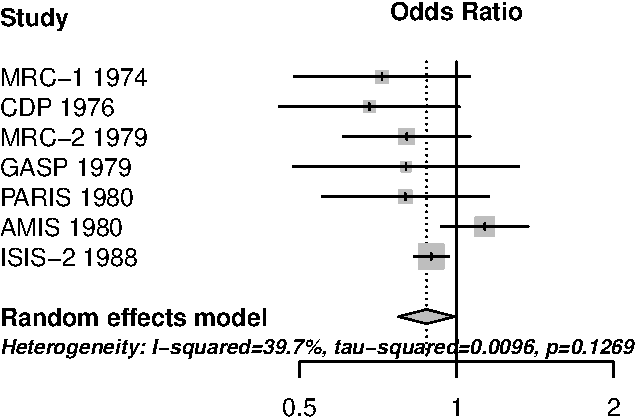
\includegraphics{./meta_files/figure-latex/unnamed-chunk-4.pdf}

\begin{Shaded}
\begin{Highlighting}[]
\KeywordTok{funnel}\NormalTok{(m1)}
\end{Highlighting}
\end{Shaded}

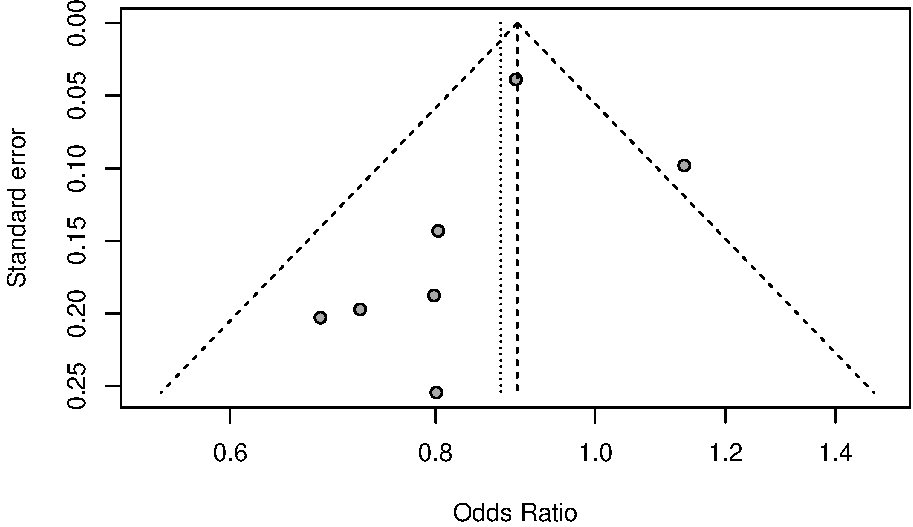
\includegraphics{./meta_files/figure-latex/unnamed-chunk-5.pdf}

\end{document}
